\documentclass[13pt]{article}
%\special{papersize=8.5in, 11in}
\usepackage[margin=1in]{geometry}
\usepackage{fancyhdr}
\usepackage[noindentafter]{titlesec}
\usepackage[T1]{fontenc}
\usepackage[scaled]{helvet}
\usepackage[pdftex]{graphicx}
\usepackage{hyperref}
\usepackage{multicol}
%\usepackage{minitoc}
\usepackage{etoc}
\usepackage{stfloats}
\usepackage{float} 
\usepackage[font=bf]{caption}
\usepackage{subfiles}
\usepackage{framed}
\usepackage{fancybox}
\usepackage{grffile}

\graphicspath{{Images//}}
% set fond
\renewcommand*\familydefault{\sfdefault}
\sffamily

\pagestyle{fancy}
\renewcommand{\footrulewidth}{0.4pt}
% define page header/footer
\lhead{}
\chead{}
\rhead{Space Shuttle Ultra Manual\\ Rev. B}
\lfoot{}
\cfoot{\thepage}
%\rfoot{\leftmark\\ \rightmark}

\titleformat*{\subsection}{\bfseries\center}
\titleformat{\paragraph}[hang]{\bfseries}{\theparagraph}{1em}{}
%\newcommand{\paragraphbreak}{\vspace{1em}}

\newcommand{\NOTE}[1]{
  \begin{center}
    \textbf{NOTE} \\
    {#1}
  \end{center}}
\newcommand{\CAUTION}[1]{
  \begin{framed}
    \begin{center}
      \textbf{CAUTION} \\
    \end{center}
    {#1}
  \end{framed}
}
\newcommand{\WARNING}[1]{
  \doublebox{
    \begin{minipage}{1.0\linewidth}
      \begin{center}
        \textbf{WARNING} \\
      \end{center}
      {#1}
    \end{minipage}
  }
}


\begin{document}
%\dosecttoc
\pagenumbering{roman}
\begin{titlepage}

\begin{center}

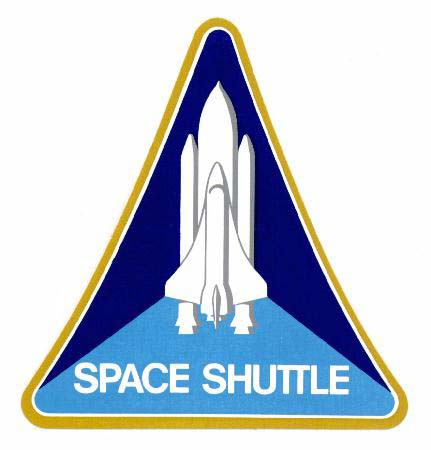
\includegraphics[width=0.35\textwidth]{SSP.jpg}\\[1cm]    

\textsc{\LARGE Space Shuttle Ultra}\\[1.5cm]

\textsc{\Large Version 1.XX  Rev. B}\\[0.5cm]

\huge \bfseries SSU Operations Manual\\[0.4cm]

\vfill

{\large \today}

\end{center}

\end{titlepage}
\begin{multicols}{2}
\section*{\large PREFACE}
%\addcontentsline{toc}{section}{PREFACE}
Space Shuttle Ultra (SSU) is an addon for Orbiter Space Flight Simulator.  The purpose of this addon is to fully simulate the NASA's Space Transportation System Program.  Currently only a few elements have been completed and work on others is ongoing.\\
\\
The basis for this addon was the Space Shuttle Deluxe but through adding additional subsystems and taking full advantage of the 2010 version of Orbiter, the current SSU has few similarities to the original Deluxe.  Currently, SSU simulates a number of systems, displays, and procedures of the real shuttle and can be used along with real NASA Flight Data File (FDF) checklists to complete tasks.  These checklists can be found at \url{http://www.nasa.gov/centers/johnson/news/flightdatafiles/index.html}, and provide a good reference for other procedures.\\
\\
Other good NASA references are the Shuttle Crew Operations Manual (SCOM), the DPS Dictionary, and the various Workbooks and Handbooks that are available on the Internet (these can also be found at the above link). \\
\\
This document contains the condensed material taken from various NASA documents as well and Orbiter and SSU specific information.  The goal of this document is to provide a typical Orbiter User the information need to perform basic SSU flights as well as  to aid in basic custum mission creation.  Separate documents will be provided for developers who would like to create a SSU compatible payloads and scenarios.\\
\\
This document is formated to look the same as the SCOM to facilitate changing from one document to the other.  Additional information or clarification is presented in three formats: notes, cautions, and warnings. Notes provide amplifying information of a general nature. Cautions provide information and instructions necessary to prevent hardware damage or malfunction (not yet simulated). Warnings provide information and instructions necessary to ensure crew safety (also not simulated). The formats in which this material appears are illustrated below.\\
\\
\NOTE{A barberpole APU/HYD READY TO START talkback will not inhibit a start.}
\CAUTION{After an APU auto shutdown, the APU FUEL TK VLV switch must be taken to CLOSE prior to inhibiting auto shutdown logic. Failure to do so can allow the fuel tank isolation valves to reopen and flow fuel to an APU gas generator bed that is above the temperature limits for safe restart.}
\WARNING{The FUEL CELL REAC switches on panel R1 are in a vertical column with FUEL CELL 1 REAC on top, FUEL CELL 3 REAC in the middle, and FUEL CELL 2 REAC on the bottom. This was done to allow the schematic to be placed on the panel. Because the switches are not in numerical order, it is possible to inadvertently close the wrong fuel cell reactant valve when shutting down a fuel cell.}
\end{multicols}

\newpage
\tableofcontents
\newpage

\pagenumbering{arabic}
\begin{multicols}{2}
\section{\large GENERAL DESCRIPTION}
%\secttoc
\localtableofcontents
%\begin{tabular}{|p{6.9cm}  p{0.25cm}|}
%	\hline
%	&\\[0.1cm]
%	CONTENTS & \\[0.4cm]
%	1.1	OVERVIEW & 2\\
%	1.2	ORBITER AND SSU & 7\\
%	1.3	COMPONENTS OVERVIEW & 10\\
%	\hline
%\end{tabular}
%\\[0.4cm]
\noindent
The section provides general background information about the obiter, its configuration and coordinate system, the nominal mission profile, and general procedures followed during a shuttle mission. It also briefly discusses components, such as the external tank and solid rocket, that are not included in the next section on orbiter systems.\\
\\
Also included in this section is keyboard commands for SSU but will not include standard Orbiter keyboard commands. See Orbiter.pdf for standard Orbiter keyboard commands.
\newpage

\subsection{\large OVERVIEW}
\localtableofcontents
%\begin{tabular}{|p{6.9cm} p{0.25cm}|}
%	\hline
%	&\\[0.1cm]
%	CONTENTS & \\[0.4cm]
%	Space Shuttle Overview & 2\\
%	Nominal Mission Profile & 2\\
%	Launch and Landing Sites & 4 \\
%	Shuttle Location Codes &  4\\
%	\hline
%\end{tabular}

\end{multicols}
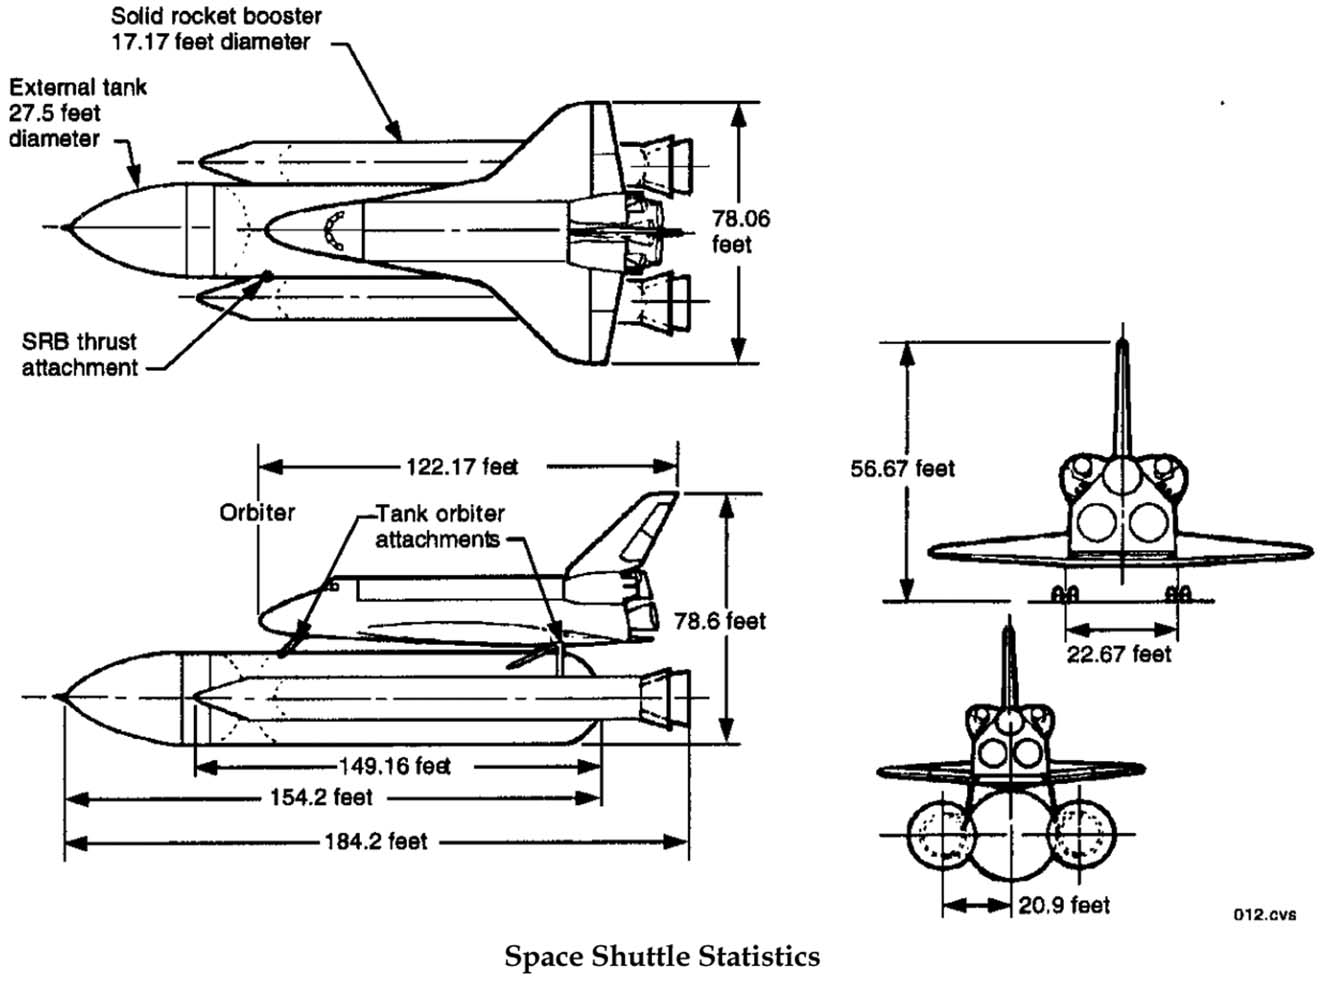
\includegraphics[width=1\textwidth]{Space Shuttle Stats.jpg}
\begin{multicols}{2}

%\subsection*{\large Space Shuttle Overview}
%\subsubsection{\large Space Shuttle Overview}
%\addcontentsline{toc}{subsection}{Space Shuttle Overview}
\noindent
The space shuttle system consists of four primary elements: an orbiter spacecraft, two solid rocket boosters (SRBs), and external tank (ET) to house fuel and oxidizer, and three space shuttle main engines (SSMEs). The shuttle can transport payloads into near Earth orbit 100 to 312 nm (185 to 577 km) above the Earth. Payloads are carried in a bay 15 feet in diameter and 60 feet long. Major system requirements are that the orbiter and the two SRBs be reusable.\\
\\
The orbiter has carried a flight crew of up to eight persons. The nominal mission is 4 to 16 days in space. The crew compartment has a shirtsleeve environment, and the acceleration load is never greater than 3 g's. In its return to Earth, the orbiter has a crossrange maneuvering capability of about 1,100 nm.\\

\subsubsection{\large Nominal Mission Profile}
%\addcontentsline{toc}{subsection}{Nominal Mission Profile}
SSU has reached a point of development that almost a full mission profile can be simulated. Continued development of Entry, from Entry Interface (EI) to terminal area energy management (TAEM), will see implementation of the entry guidance and displays that will aid in executing reentry but for now it must be done manually with limited instrumentation.\\
\\
\paragraph{Launch}
In launch configuration, the orbiter and two SRBs are attached to the ET in a vertical (nose-up) position on the launch pad.\\
\\
The three SSMEs, fed liquid hydrogen fuel and liquid oxygen oxidizer from the ET, are ignited first $\sim$T-6 seconds. Once proper operation and thrust level has been varified, a signal is sent at T-0 seconds to the SRBs which ignite and the stack is released from the launch pad.\\
\\
After approximately 2 minutes into the ascent phase, the two SRBs have consumed their propellant and are jettisoned from the ET. This is triggered by a separation signal from the orbiter.\\
\\
The orbiter and ET continue on to orbit while the SRBs begin to descend back to Earth. At a predetermined altitude, parachutes are deployed and the boosters spashdown in the ocean.
The boosters are recovered and reused.\\
\\
After approximately 8 and a half minutes after launch, the three main engines undergo main engine cutoff (or MECO), and the ET is jettisoned on command from the orbiter.\\
\\
The forward and aft reaction control system (RCS) jets provide attitude control, translate the orbiter away from the ET at separation, and maneuver the orbiter to burn attitude prior to the orbital maneuvering system (OMS) burn. The ET continues on a ballistic trajectory and enters the atmosphere, where it disintegrates.\\
\\
\paragraph{Orbit Insertion and Circularization}
The nominal ascent profile, referred to as "direct insertion," places the vehicle in a temporary elliptical orbit at MECO. Orbital altitudes can very depending on mission requirements. The crew performs an OMS burn, designated as ``OMS 2'', to stabilize the orbit. This burn can add anywhere between 200 to 550 fps to the vehicle's orbital velocity, as necessary.\\
\\
In cases of severe performance problems during the ascent, the vehicle may find itself well short of the expected MECO velocity, and even suborbital. In such cases, the crew performs what is call an ``OMS 1'' burn shortly after MECO, which raises the orbit to a safe altitude. They then perform an OMS 2 burn to stabilize that orbit.\\
\\
When simulating early missions with SSU, the orbiter will perform what was known as a ``standard insertion''. This will place the orbiter in a heads down suborbital orbit at MECO and will require an OMS 1 burn.  This ascent profile was used for the first ten missions, STS-1 though STS-41B.\\
\\
\paragraph{Orbit}
On orbit, the forward and aft RCS jets provide attitude control of the orbiter, as well as any minor translation maneuvers along a given axis. The OMS engines are used to perform orbital transfers, such as those done to rendezvous with the International Space Station (ISS). Mission objectives while in orbit has ranged from ISS assembly and logistics, payload deployment and retrieval, to scientific experiments.  Also several planed, but not flown, missions are planed to be simulated with SSU including shuttle-Centaur flights and posible Vandenberg missions.
\\
\paragraph{Deorbit}
At the completion of orbital operations, the RCS is used to orient the orbiter in a tail-first attitude. The two OMS engines are burned to lower the orbit such that the vehicle enters the atmosphere at a specific altitude and range from the landing site. The deorbit burn usually decreases the vehicle's orbital velocity anywhere from 200 to 550 fps, depending on orbital altitude.  When the deorbit burn is complete, the RCS is used to rotate the orbiter's nose forward for entry. The RCS jets are used for attitude control until atmospheric density is sufficient for the pitch, roll, and yaw aerodynamic control surfaces to become effective.
\\
\paragraph{Entry}
Orbiter reentry is normally controlled automatically by the Aerojet Digital Autopilot (DAP) from entry interface (EI) through TAEM, to $\sim$ Mach 1, where the CDR takes control of the orbiter. SSU has a fully functioning entry autopilot which provides guidance and control from EI to Mach 2.5 (the start of TAEM). It is also possible to fly the shuttle manually.
\\
\paragraph{TAEM}
TAEM (terminal area energy management) guidance steers the orbiter to one of two heading alignment cones (HAC), which are located to and on either side of the runway centerline on the approch end. In real lift, the shuttle is flown on autopilot from the start of TAEM up to $\sim$ Mach 1, when the CDR takes control and manually flies the shuttle to landing. The autopilot for the TAEM phase has not been implemented; however, guidance commands are displayed on the HUD. Detailed desriptions will be included later in this document.
\\
\paragraph{Landing}
Approach and landing easily performed without TAEM guidance. After runway acqusition on rollout from the HAC one can visually fly the orbiter to runway. Detailed desriptions of final approach and landing will be included later in this document.\\

\subsubsection{\large Launch and Landing sites}
%\addcontentsline{toc}{subsection}{Launch and Landing sites}
During the Shuttle program, The Kennedy Space Center (KSC) in Florida was used for all shuttle launches. Currently in SSU that is also true. Eventually, SSU hopes to simulate West Coast shuttle operations based at Vandenberg Air Force Base as it was originaly planned until the Challenger accident in 1986. Shuttle landings occur at KSC, also, as well as at Edwards Air Force Base in California. Contingency landing sites are also provided in the event the orbiter must return to Earth in an emergency.\\
\\
\begin{tabular}{c}
	\bfseries NOTE\\[0.3cm] KSC is currently the only base that is\\ included with SSU.  Eventually Edwards,\\ White Sands, VAFB, and the abort\\ landing sites will be included.
\end{tabular}
\\[0.5cm]
A 035$^{\circ}$ azimuth launch places the spacecraft in an orbital inclination of 57$^{\circ}$, which means the spacecraft in its orbital trajectories around Earth will never exceed an an Earth latitude higher or lower than 57$^{\circ}$ north or south of the equator. A launch path from KSC at an azimuth of 090$^{\circ}$ (due east from KSC) will place the spacecraft in an orbital inclination of 28.5$^{\circ}$.
\\
These two azimuths, 035$^{\circ}$ and 090$^{\circ}$, represent the current launch limits from KSC. Any azimuth angles further north or south would launch the spacecraft over a habitable land mass, adversely affect safety provisions for abort or vehicle separation conditions, or present the undesirable possibility that the SRB or external tank could land on inhabited territory.
\\
\subsubsection{\large Shuttle Location Codes}
%\addcontentsline{toc}{subsection}{Shuttle Location Codes}
Orbiter location codes enable crewmembers to locate displays and controls, stowage comparments and lockers, access panels, and wall-mounted equipment in the orbiter crew compartments. The crew compartments are the flight deck, middeck, and airlock. Because of compartment functions and geometry, each has a unique location coding format.
\\
Currently SSU only simulates the flight deck to the degree that location coding must be followed. Soon panels in the middeck will be simulated and at that time the middeck location coding will be included in this manual.
\\
\paragraph{Flight Deck Location Codes}
A flight deck location code consists of two or three alphanumeric characters. The first character is the first letter of a flight dect surface as addressed while sitting in the commander/pilot seats. The characters are:
\\
\begin{tabular}{r c l}
	L& - &Left\\
	R& - &Right\\
	F &-& Forward\\
	A &-& Aft\\
	C &- &Center Console\\
	O &-& Overhead\\
	S &-& Seats\\
	W &-& Window\\
\end{tabular}
\\
\end{multicols}
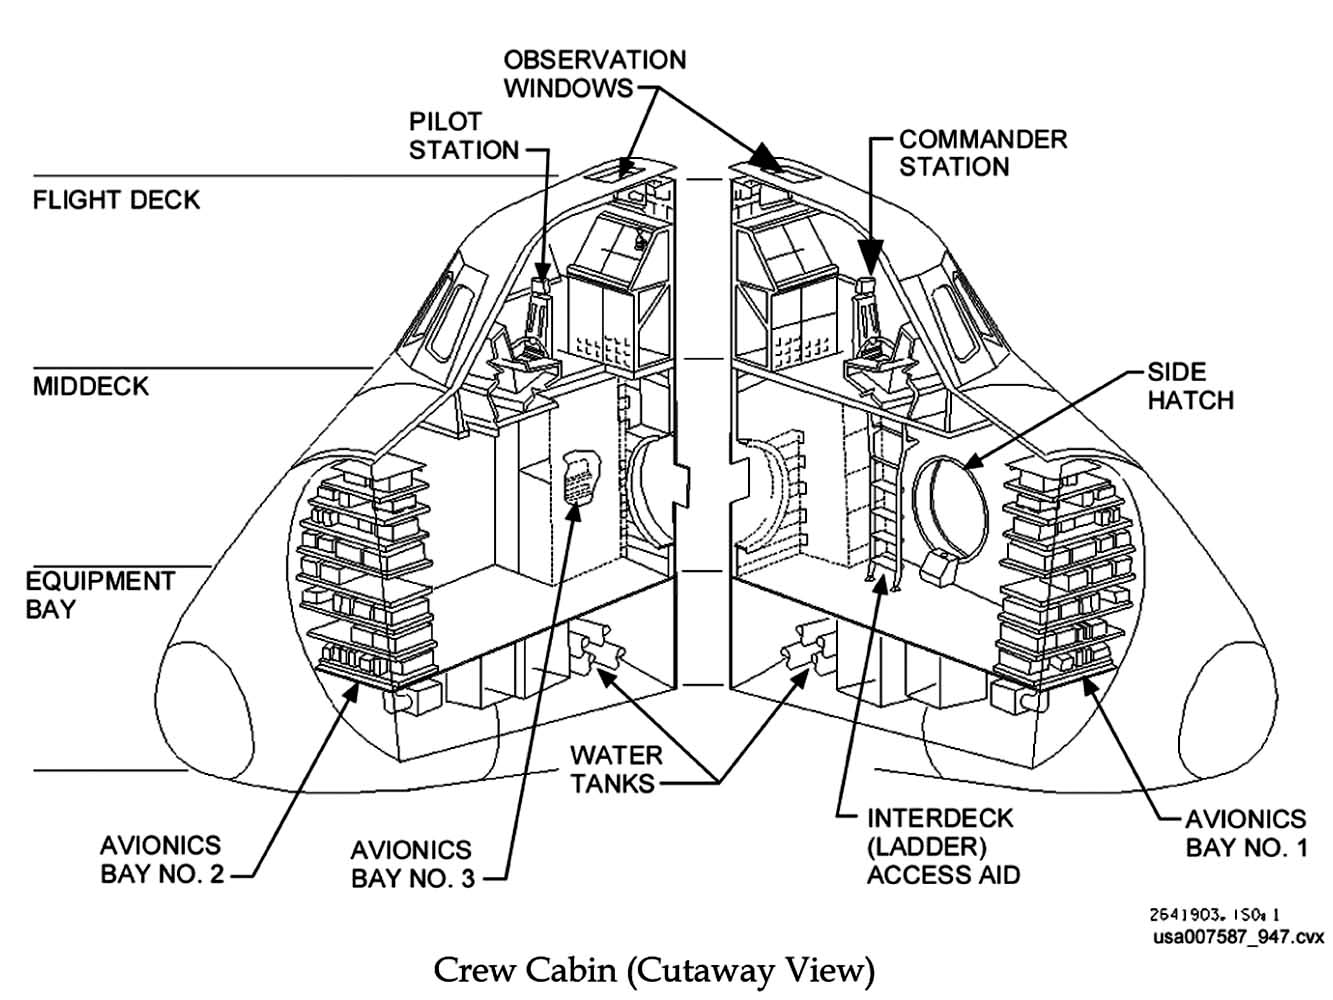
\includegraphics[width=0.85\textwidth]{Crew Cabin (Cutaway).jpg}
\begin{multicols}{2}
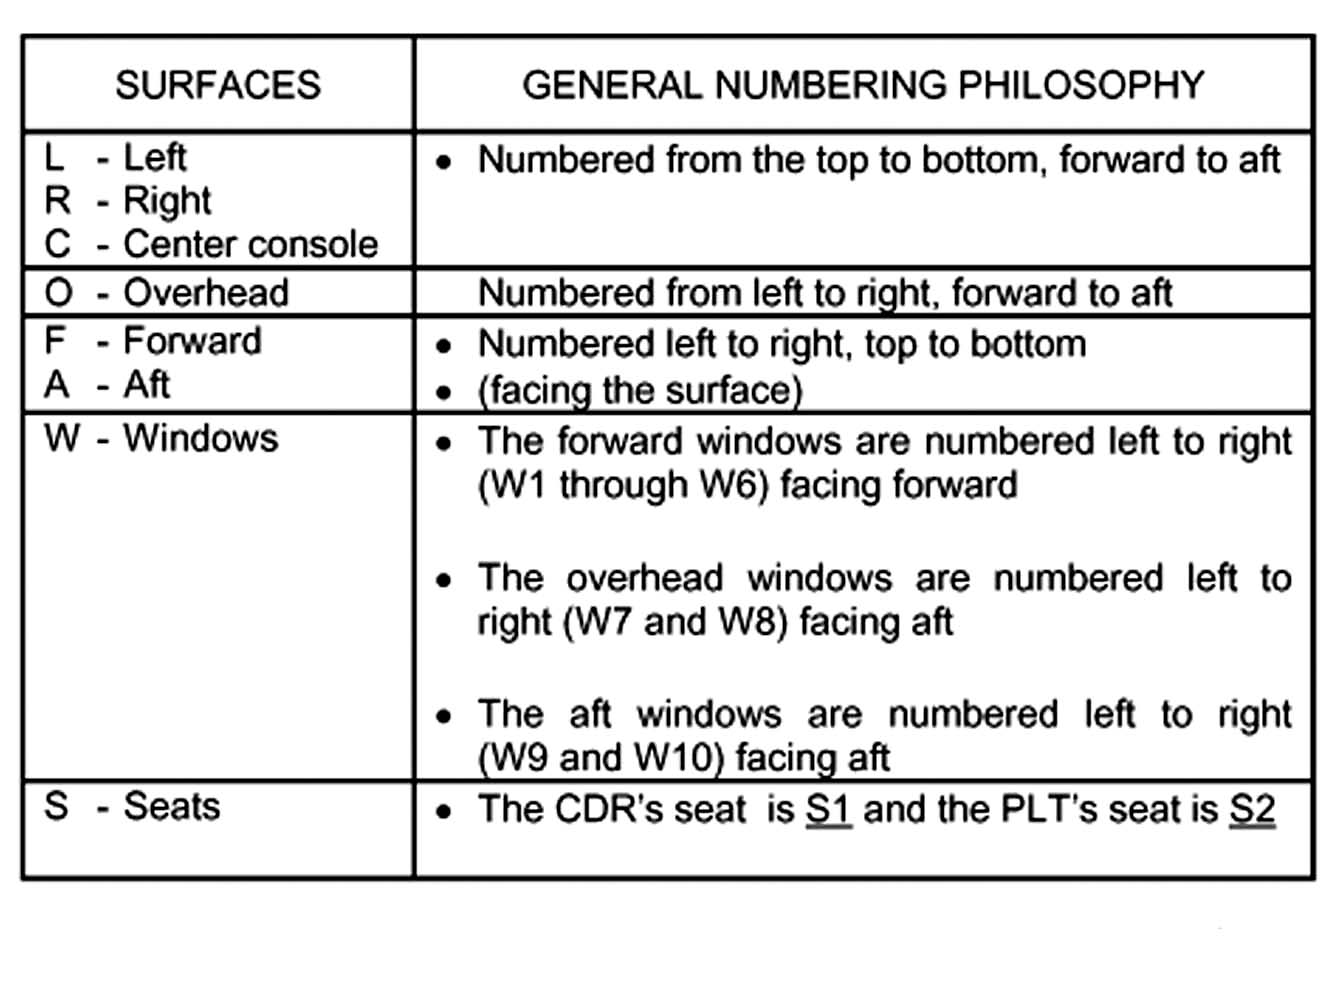
\includegraphics[width=0.45\textwidth]{FD_Codes_Chart.jpg}
The second and third characters are numerics identifying the relative location of componets on each flight deck surface. The numbering system philosophy is summerized in the table at left.
\\
\end{multicols}
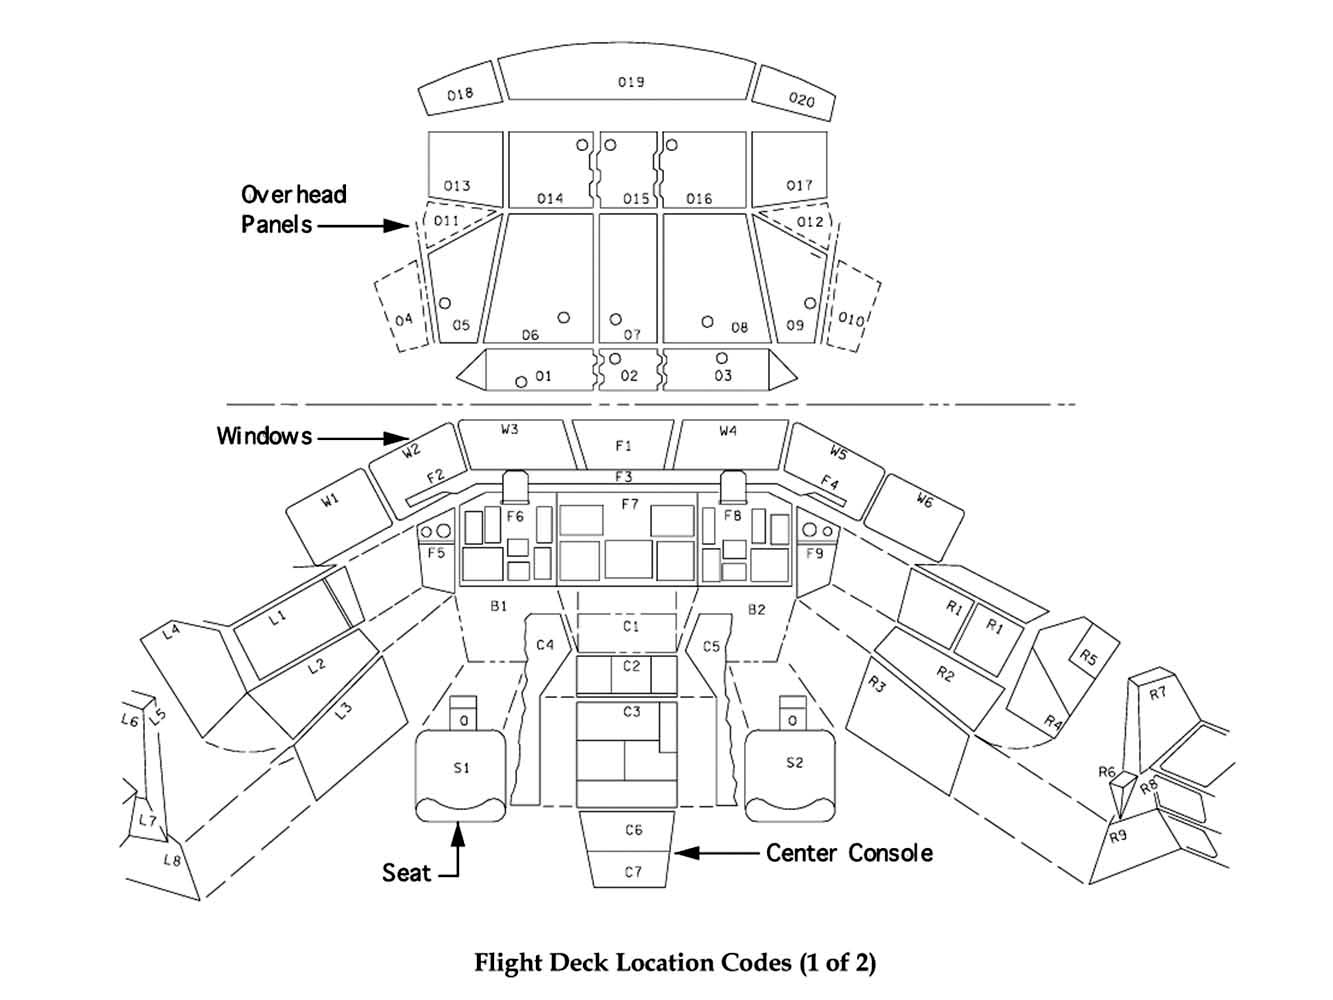
\includegraphics[width=1\textwidth]{Flight_Deck_Loc_Codes_1.jpg}

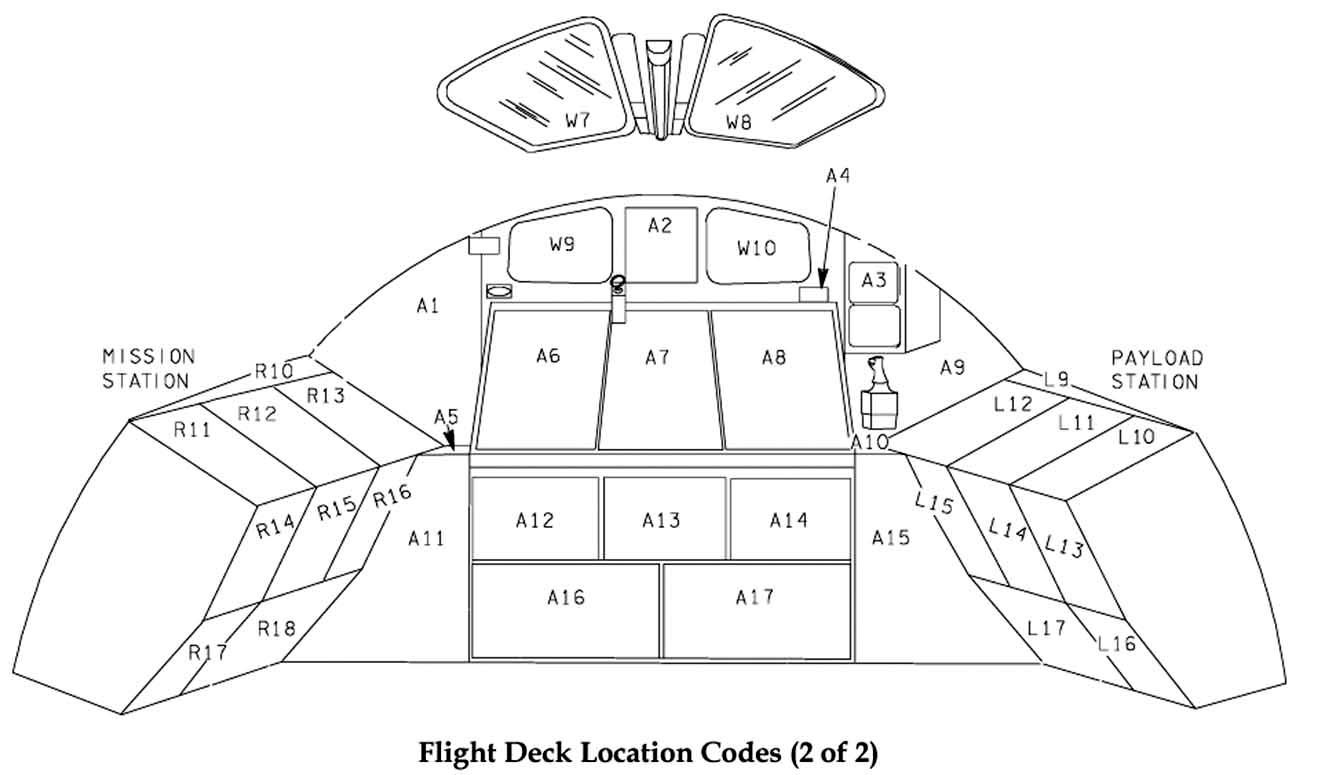
\includegraphics[width=1\textwidth]{Flight_Deck_Loc_Codes_2.jpg}

\vfill

\newpage
\subsection{\large ORBITER AND SSU}
\localtableofcontents
%\begin{tabular}{|p{7cm} p{0.25cm}|}
%	\hline
%	&\\[0.1cm]
%	CONTENTS & \\[0.4cm]
%	SSU Keyboard Commands & 7\\
%	Camera Views & 8\\
%	Payload Operations Overview & 9\\
%	\hline
%\end{tabular}


\subsubsection{\large SSU Keyboard Commands}
%\addcontentsline{toc}{subsection}{SSU Keyboard Commands}
The ultimate goal of SSU is to provide a complete simulation of the Space Shuttle.  This means that most of the imput is done with in-simulation controls (ie. cockpit switches, GNC keyboards, and dialog windows). This results in very few keyboard commands to operate the shuttle.

\paragraph{General}
Ctrl+A - toggle between controlling RCS thrusters and RMS motion\\
Ctrl+G - arm landing gear\\
G - deploy landing gear\\
comma - open speedbrake by 5 percent\\
period - close speedbrake by 5 percent\\

\paragraph{Alternate Translation Commands (valid only if RCS is in Rot mode)}
Left/Right Arrow - left/right translation (equivalent to 1/3 on Numpad)\\
Up/Down Arrow - up/down translation (equivalent to 8/2 on Numpad)\\
Insert/Delete - forward/aft translation (equivalent to 9/6 on Numpad)\\

\paragraph{RMS}
Ctrl+Enter - grapple\\
Ctrl+Backspace - release\\
Ctrl+O - toggle between Coarse and and Vern rates\\

\begin{multicols}{2}
\subsubsection{\large RHC/THC}
The regular Orbitersim thruster control commands (either keyboard or joystick) are used to simulate the RHC \& THC. When controlling the RCS thrusters, the appropiate \textit{FLT CNTLR PWR} switch must be on for RHC/THC inputs to be used. There are no such restrictions when controlling the RMS (although the RMS needs to be powered on before it can move).
\\
\\
The RHCs on the real shuttle have a "soft stop" and a "hard stop" (the mechanical limit of movement). Moving the RHC out of detent (up to the soft stop) will command either a constant rotation rate or a pulse of RCS firings to change the rotation rate by a specified amount (depending on whether \textit{DISC RATE} or \textit{PULSE} has been selected). Moving the RHC past the soft stop will result in continuous thruster firings in the appropriate axis. In SSU, a thruster command of <75\% is considered to be within the soft stop; a thruster command of >75\% is treated as RHC deflection beyond the soft stop. When using keyboard controls, the normal keyboard controls are equivalent to full RHC deflection, while holding down the Ctrl key is equivalent to deflection within the soft stop. The THC (and the RMS controls) does not have this idea of a soft stop. When \textit{NORM} is selected in a translational axis, the thrusters will fire continuously if the THC is moved out of detent. When \textit{PULSE} is selected, the thrusters will fire to provide a specified DeltaV (the TRAN PLS rate specified on the SPEC 20 DAP CONFIG display). When controlling the RMS, the commanded rotation/translation rates are always directly proportional to the RHC/THC deflection.

\subsubsection{\large Speedbrake/Thrust Controller}
On the real shuttle, the Speedbrake/Thrust Controller (SBTC) controls both SSME throttling during ascent and the speedbrake during entry. In Orbiter, the SBTC is simulated using the main engine key controls. The Orbitersim throttle setting is mapped to the SBTC range. During ascent, 0\% Orbitersim main thrust corresponds to 67\% SSME throttle; 100\% Orbitersim main thrust corresponds to 104.5\% (109\% during some abort cases) SSME thrust. During entry, 0\% main thrust corresponds to the speedbrake being \textbf{fully open}; 100\% main thrust corresponds to the speedbrake being commanded \textbf{fully closed}.

\paragraph{Ascent}
During ascent, SSME throttling is usually controlled by autopilot; in this case, the \textit{AUTO} portion of the \textit{SPD BK/THROT} PBIs on Panel F2 \& Panel F4 is lit. To takeover manual control, move the SBTC (by changing the Orbitersim main engine throttle) to match the current autopilot command. At this point, both \textit{AUTO} PBIs will go out and the PLT \textit{SBD BK/THROT MAN} PBI will be lit (the CDR PBI will not be lit; in real life, only the PLT SBTC can be used during ascent, although SSU allows the SBTC to be used from both CDR and PLT seats). MECO is commanded by pressing the NUMPAD * key (in real life, this is done by simultaneously pressing all 3 \textit{MAIN ENGINE SHUT DOWN} pushbuttons on Panel C3; this is not possible in Orbiter).

\paragraph{Entry}
The speedbrake is usually controlled automatically throughout entry. To take over manual control move the SBTC; the speedbrake will immediately move to the position commanded by the SBTC and the \textit{AUTO} portion of the \textit{SPD BK/THROT} PBIs will go out and the \textit{MAN} PBI will be lit on either the CDR or PLT position (depending on the current VC position). Pressing the \textit{SPD BK/THROT} PBI will but the speedbrake into \textit{AUTO} mode again.

%\newpage

\subsubsection{\large Camera Views}
%\addcontentsline{toc}{subsection}{Camera Views}
SSU includes the four payload bay cameras and the docking port centerline camera. The PLB cameras are controled via their switches on panel A7U on the flight deck and are no longer controled with a dialog window. In the PLB camera VC views, the cameras can be rotated using ALT+Arrow Key.

\paragraph{Navigating the Virtual Cockpit}
Changing between Virtual Cockpit (VC) views is identical to the system used in the default Atlantis but with several more positions around the cockpit that we call stations. You can switch between different stations using the Ctrl+Arrow key combination (See Chart below for all combinations.) The Commander (CDR) Station is the front left seat on the flight deck, while the Pilot (PLT) station is the right seat (while looking forward).\\

The table below is set up to show the different ways to move about the crew module. The first column is the camera position you are in and the other columns show the views you can change to using the Ctrl+Arrow key combination at the top of the table. For additional assistance in navigating the views, the name of the view is shown for a few seconds at the top of the screen during the simulation. The names in the table are identical to those that appear on-screen.\\
\end{multicols}
\begin{tabular}{|l|l|l|l|l|}
	\hline
	Cockpit View & Left & Right & Up & Down \\
	\hline \hline
	Commander Seat & Port Workstation & Pilot Seat & ODS Camera & MS Seat \\
	\hline
	Pilot Seat & Commander Seat & Stbd Workstation & ODS Camera & MS2/FE Seat \\
	\hline
	MS Seat & Port Workstation & MS2/FE Seat & Commander Seat & ODS Camera\\
	\hline
	MS2/FE Seat & MS Seat & Stbd Workstation & Pilot Seat & ODS Camera\\
	\hline
	Port Workstation & RMS Work Station & Commander Seat & ODS Camera & Middeck\\
	\hline
	Stbd Workstation & Pilot Seat & Aft Pilot Station & ODS Camera & Aft Workstation\\
	\hline
	Aft Workstation & Stbd Workstation & Port Workstation & RMS Work Station & MS Seat\\
	\hline
	Aft Pilot Station & Stbd Workstation & RMS Work Station & ODS Camera & Aft Workstation\\
	\hline
	RMS Work Station & Aft Pilot Station & Port Station & ODS Camera & Aft Workstation\\
	\hline
	RMS EE & RMS Elbow & - & - & RMS Work Station\\
	\hline
	RMS Elbow & - & RMS EE & - & RMS Work Station\\
	\hline
	PLB Camera A & PLB Camera D & PLB Camera B & RMS EE & ODS Camera\\
	\hline
	PLB Camera D & PLB Camera C & PLB Camera A & RMS EE & ODS Camera\\
	\hline
	PLB Camera B & PLB Camera A & PLB Camera C & RMS EE & ODS Camera\\
	\hline
	PLB Camera C & PLB Camera B & PLB Camera D & RMS EE & ODS Camera\\
	\hline
	ODS Camera & - & - & PLB Camera D & Aft Pilot Station\\
	\hline
\end{tabular}
\newpage
\subsection{\large Payload Operations Overview}
%\addcontentsline{toc}{subsection}{ Payload Operations Overview}
Payloads are attached through standard Orbiter attachment points. The diagram below will assist in visializing the available attachment locations.\\
\\
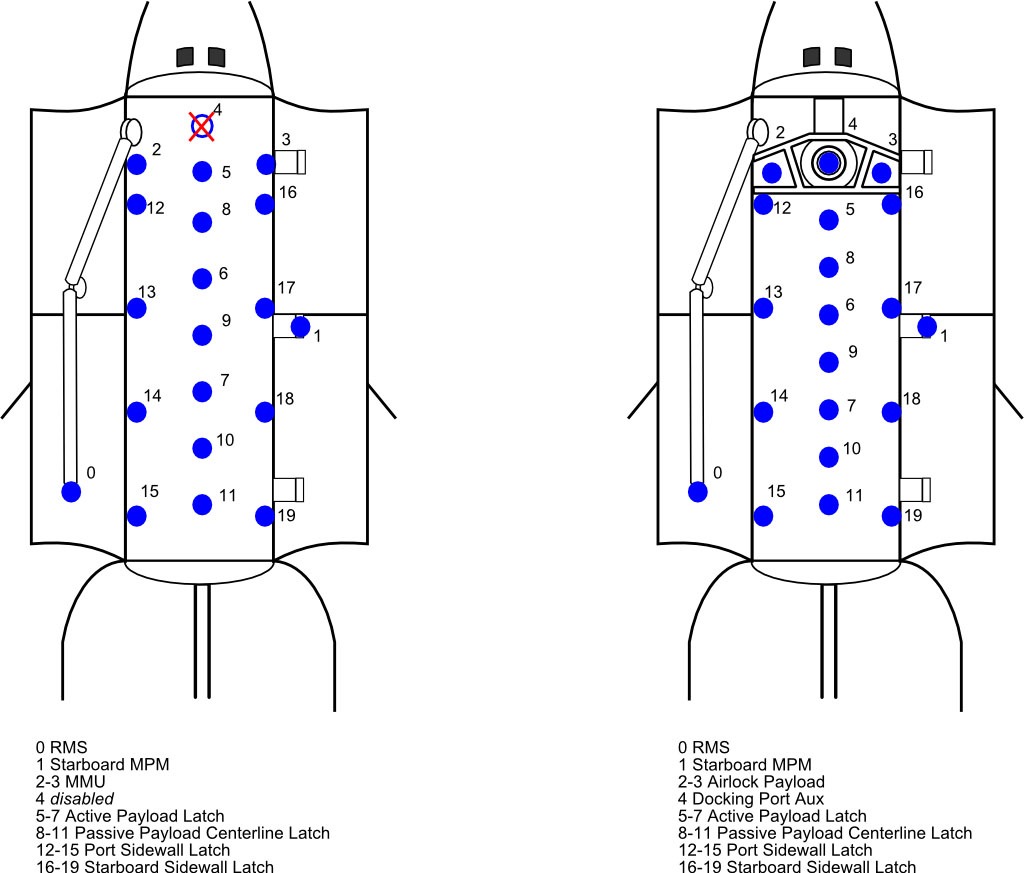
\includegraphics[width=1\textwidth]{SSU_Attachments.png}
\\
\\
\\
\\
Currently no payload bay bridgerails are shown, this makes payload berthing in the bay difficalt at best.  If the payload is one that is deployed and later put back into the bay (example: MPLM), be sure to take note of the SRMS joint angles and orbiter XYZ coordenents displayed on panel A8U. For more information on the payload deploment and retreval systems see section 2.9. The scenario file entries needed to add payloads to SSU are covered in section 5 of this manual. \\
\\
\newpage
\begin{multicols}{2}
%\subsection{\large Components Overview}
%\localtableofcontents
%\begin{tabular}{|p{7cm} p{0.25cm}|}
%	\hline
%	&\\[0.1cm]
%	CONTENTS & \\[0.4cm]
%	Orbiter & 10\\
%	External Tank & 11\\
%	Solid Rocket Boosters & 11\\
%	\hline
%\end{tabular}
\subsection{\large Orbiter}
\localtableofcontents
%\addcontentsline{toc}{subsection}{ Orbiter}

The Orbiter is the manned vehicle component of the Space Shuttle System and is the only component to reach orbital velocities.  The orbiter itself is divided into nine major sections: (1) forward fuselage, which includes the crew compartment, (2) wings, (3) midfuselage, (4) payload bay doors, (5) aft fuselage, (6) forward RCS, (7) vertical tail, (8) OMS/RCS pods, (9) body flap.  Many of these sections are only structural sections of the orbiter and are thus not simulated by SSU. The following descriptions discuss the key sections as they pertain to the user in simulation and point out important systems contained in them.


\subsubsection{Forward Fuselage}
The forward fuselage contains the crew compartment, forward RCS module, nose cap, nose gear wheel well with associated gear and doors.  The forward fuselage also contains various antennas, deployable air data probes and the openings for the two star trackers.
\\

\subsubsection{Crew Compartment}
The crew compartment arrangement consists of three levels, the flight deck, the middeck and the lower equipment bay. Currently only the flight deck and the middeck are simulated in any capacity. The compartment has a side hatch for normal ingress and egress, a hatch into the airlock from the middeck, and a hatch from the airlock into the payload bay for extravehicular activity and payload bay access (Currently none of these hatches are simulated).

\end{multicols}
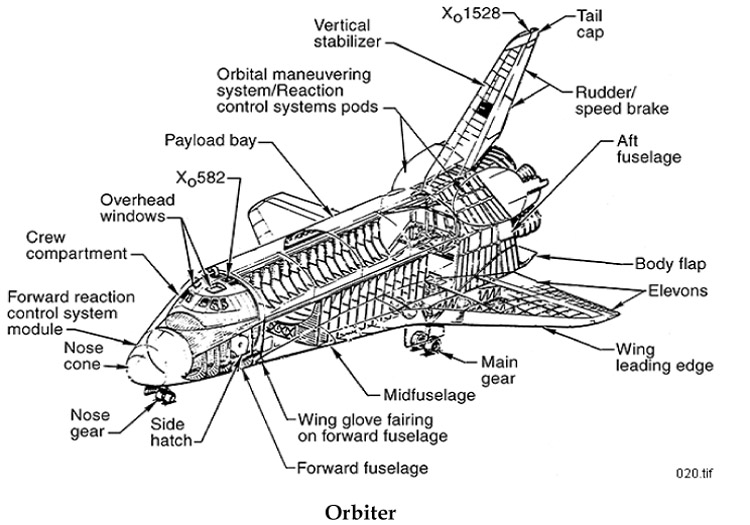
\includegraphics[width=1\textwidth]{Orbiter.jpg}

\newpage
\begin{multicols}{2}
\subsubsection{Flight Deck}
The fight deck is the uppermost compartment in the cabin.  The flight deck is further divided into two halves. The forward flight deck has the commander and pilot work stations and contains controls and displays for controlling the vehical throughout all mission phases. The aft flight deck, the rear section of the deck, contains displays and controls for orbital maneuvers, rendezvous maneurvers, stationkeeping, docking, payload deployment and retrival, playload monitoring, remote manipulator system controls and displays, payload bay door operations, and CCTV operations.  Currently all operations that can be done with SSU are done from the flight deck.

\subsubsection{Midddeck}
The middeck contains areas for crew life on-orbit.  While some switches that are required to operate equipment on the flight deck are located here, SSU currently does not simulate these switches.  The middeck is modeled and can be entered in the VC but thereare no funtions to be performed there currently.
\\

\subsubsection{Midfuselage}
The midfuselage contains the payload bay, payload bay doors, main landing gear wells and gear, fuelcell equipment, and attachment structure for the wings. For SSU, this is where payloads are attached to the orbiter and where most of the PDRS and EVA activity is located. See these system sections for detailed information about systems contained in the midfuselage: 
% TODO: cross-reference these
\begin{itemize}
\item 2.6 Mechanical Systems
\item 2.8 Orbiter Docking System
\item 2.10 Payload Deployment and Retieval System
\end{itemize}
\subsubsection{Aft Fuselage \& OMS/RCS Pods}
The aft fuselage holds systems including the APUs, Water Spray Boilers, and the three SSMEs. It also provides attachment structure for the vertical stabilizer, body flap, and the OMS/RCS pods.  The aft OMS/RCS system is interconnected between the left and right pods.
\newpage
\subsection{\large External Tank}
%\addcontentsline{toc}{subsection}{ External Tank}
The external tank (ET) contains the liwuid hydrogen and liquid oxygen oxidizer and supplies them under pressure to the three SSMEs in the orbiter during ascent. When the SSMEs are shut down, the ET is jettisoned and enters the Earth's atmosphere, where it breaks up and inpacts in a remote ocean area.\\
\\
The ET itself is made up of three main elements, an Oxygen tank, an unpressurized intertank, and a hydrogen tank.  The ET makes up the backbone of the STS stack and provides attachment interfaces for the two Solid Rocket Boosters.\\
\\
Because SSU means to simulate historical missions, the different types of ETs have been simulated. The earliest tank used on STS-1 through STS-5 and STS-7, is called a Standard Weight Tank (SWT). The first two of these, used on STS-1 and 2, were painted white to protect the tanks from ultraviolet light.  This was later determined to not be a problem and all later tanks were not painted removing 600 lb of weight from the tank.\\
\\
The second version of the ET was called the Lightweight Tank (LWT).  These tanks flew on mission begining with STS-6 and was last used on STS-107.  The last type of tank is the Super Lightweight Tank (SLWT).  These tanks have been used from STS-91 (STS-99 and STS-107 were exceptions) up until the end of the program.\\
\\
For SSU, the main difference between these tanks are the weight and visual appernce.  All ETs will show charred SOFI after SRB sep. Eventually, users will be able to attach the ET to the SRBs in the VAB in stacking simulations but this is still early in development and is incomplete.\\
\subsection{\large Solid Rocket Boosters}
%\addcontentsline{toc}{subsection}{ Solid Rocket Boosters}
The two Solid Rocket Boosters (SRBs) are the largest solid-propellant motors ever flown and the first ever designed for reuse.\\
\\
As with the real shuttle SSUs SRBs are attached to the launch platform during prelaunch.  Once the SSMEs have been verified operating normal, the stack is detached from the pad and the SRBs are ignited. The SRBs cannot be turned off and must remain on the vehical until burnout.\\
\\
SRB ground operations will include SRB ocean retrival and SRB segment stacking in the VAB. Stacking operations are still incomplete.

\end{multicols}
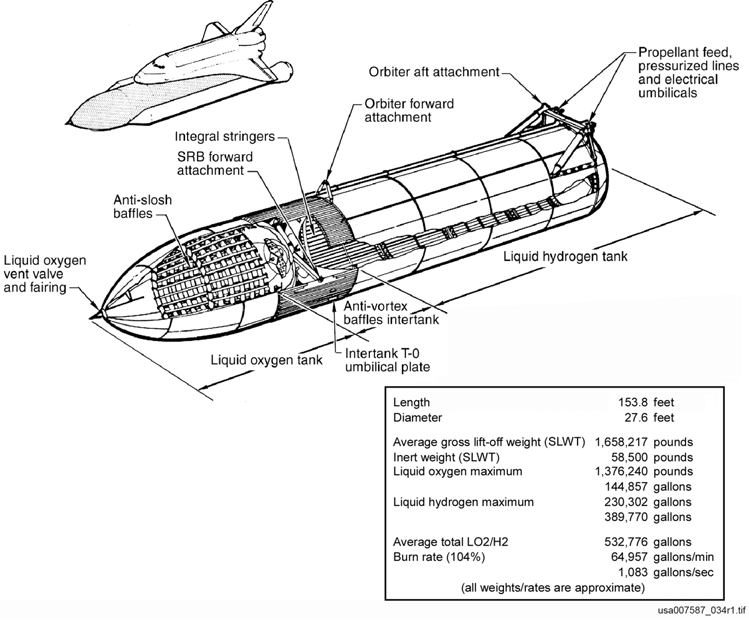
\includegraphics[width=0.85\textwidth]{SLWT.png}
\captionof*{figure}{Super Lightweight Tank (image from SCOM)}
%\\
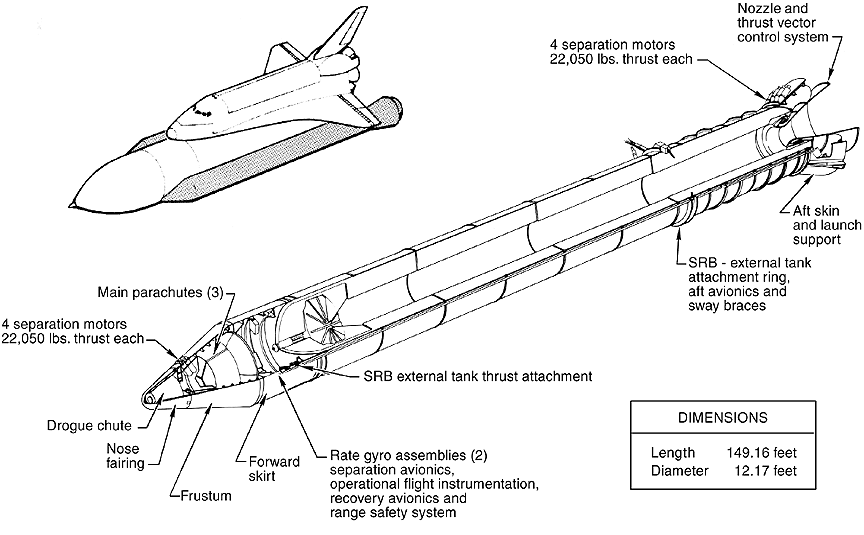
\includegraphics[width=0.85\textwidth]{SRB.png}
\captionof*{figure}{Solid Rocket Booster (image from SCOM)}


\newpage
\subfile{SSU_SYSTEMS}
\newpage
\subfile{FLIGHT_DATA_FILES}
\newpage
\subfile{MISSION_FILES}
\newpage
\subfile{SCENARIO_FILES}

\newpage
\section{\large CREDITS}
Space Shuttle Ultra was originally based on Space Shuttle Deluxe. Large parts of the launch autopilot were copied (with minor modifications) from PEG MFD.
Some of the attitude control code was derived from Attitude MFD V3.
SSU also uses the KOST library. \\
\\
This addon is open-source and is released under the GNU GPL. \\
\\
DISCLAIMER: The SSU team is not responsible for any crashes or other problems caused by this addon. Use at your own risk.
\end{document}